
\subsection[SO(2,2n-2)]{$\mathrm{SO}(2,2n-2) \sim D_n, n\geq 3$}\label{sec:conf_even}

\subsubsection{Root system data}

\[\alpha_i = \epsilon_i - \epsilon_{i+1}, i<n, \alpha_n = \epsilon_{n-1} + \epsilon_n\]
\[\omega_i = \epsilon_1+\cdots \epsilon_i, i < n-1, \quad \omega_{n-1} = \frac{1}{2}(\epsilon_1 + \cdots \epsilon_{n-1}-\epsilon_n), \quad \omega_{n} = \frac{1}{2}(\epsilon_1 + \cdots \epsilon_{n-1}+\epsilon_n)\]
\begin{align*}
 \roots &= \{ \pm \epsilon_i \pm \epsilon_j | i\neq j, i,j = 1\ldots n \} \\
 \roots_c^+ &= \{ \epsilon_i\pm \epsilon_j | 2\leq i < j \leq  n\}\\
 \roots_n^+ &= \{ \epsilon_1 \pm \epsilon_j | 2 \leq  j \leq n \}
 \end{align*}
\[\beta = \epsilon_1+\epsilon_2,\quad \rho = (n-1,\ldots ,1,0),\quad \zeta = (1,0,\ldots,0)\]
\inserttikzfigure{diagrams/dynkin_Dn_1.tikz}{Marked Dynkin diagram for $\mathrm{SO}(2,2n-2)$}

\begin{center}\begin{threeparttable}
\begin{tabular}{CCCCC}
  \text{Vertex } \lambda_a & \text{Weight } \mu_a &  Q(\lambda_a) = R(\lambda_a)& l(\lambda_a) \\ \hline
  -(2n-p-1)\omega_1+\omega_{p+1} & -(2n-p)\omega_1 + \omega_p  & \mathrm{SU}(1,p)\tnote{1} &  1 \\
  -(n+1)\omega_1 +\omega_{n-1} + \omega_n & -(n+2)\omega_1 + \omega_{n-2} & \mathrm{SU}(1,n-2) &  1 \\
  -(n-1)\omega_1 + \omega_n \tnote{2} & -n\omega_1+\omega_{n-1} &  \mathrm{SU}(1,n-1) & 1 \\
  -(n-2)\omega_1 & -n\omega_1 & \mathrm{SO}(2,2n-2) &  2\\
  0 & -2\omega_1 + \omega_2 & \mathrm{SO}(2,2n-2) &  1 \\
  -(n-1)\omega_1  + \omega_{n-1} \tnote{3} & -n\omega_1 + \omega_n &\mathrm{SU}(1,n-1) & 1
\end{tabular}\smallskip
\begin{tablenotes}
 \item [1] $1\leq p \leq n-3$ with Dynkin diagram of $R(\lambda_a)$:\\
 \begin{tikzpicture} % SO^*(2n) ~ D_n relative
	\node[nroot] (a1) [label=above:$-\beta$] {};
	\node[croot] (a2) [right= of a1] [label=above:$\alpha_2$] {};
	\node (a3) [right= of a2] {};
	\node (a4) [right= of a3] {};
	\node[croot] (a5) [right= of a4] [label=above:$\alpha_{p}$] {};
	\draw (a1) to (a2) to (a3);
	\draw [dotted] (a3) to (a4);
	\draw (a4) to (a5);
     \end{tikzpicture}
 \item [2] Dynkin diagram  of $R(\lambda_a)$:
 \begin{tikzpicture} % SO^*(2n) ~ D_n relative
	\node[nroot] (a1) [label=above:$-\beta$] {};
	\node[croot] (a2) [right= of a1] [label=above:$\alpha_2$] {};
	\node (a3) [right= of a2] {};
	\node (a4) [right= of a3] {};
	\node[croot] (a5) [right= of a4] [label=above:$\alpha_{n-1}$] {};
	\draw (a1) to (a2) to (a3);
	\draw [dotted] (a3) to (a4);
	\draw (a4) to (a5);
     \end{tikzpicture}
 \item [3] Dynkin diagram of $R(\lambda_a)$:
\begin{tikzpicture} % SO^*(2n) ~ D_n relative
	\node[nroot] (a1) [label=above:$-\beta$] {};
	\node[croot] (a2) [right= of a1] [label=above:$\alpha_2$] {};
	\node (a3) [right= of a2] {};
	\node (a4) [right= of a3] {};
	\node[croot] (a5) [right= of a4] [label=above:$\alpha_{n-2}$] {};
	\node[croot] (a6) [right= of a5] [label=above:$\alpha_{n}$] {};
	\draw (a1) to (a2) to (a3);
	\draw [dotted] (a3) to (a4);
	\draw (a4) to (a5) to (a6);
     \end{tikzpicture} 
\end{tablenotes}
\caption{Vertices and root systems for $\mathrm{SO}(2,2n-2)$, $n\geq 3$}\label{tbl:so_even}
\end{threeparttable}\end{center}

\subsubsection{Nilpotent cohomology in detail}

Scalar products of $\rho$ with positive noncompact roots
\begin{equation}\label{eq:Dn_rho_scalar_posroots}
 (\epsilon_1 + \epsilon_j, \rho) = 2n-1-j, \quad (\epsilon_1 - \epsilon_j, \rho) = j -1.
\end{equation}


\begin{enumerate}
 \item $ \lambda =  -(2n-p-1)\omega_1+\omega_{p+1}$\\
   Scalar products of positive noncompact roots with $\lambda+\rho$ are
  \begin{align*}
    (\epsilon_1 + \epsilon_j, \lambda+\rho) & = \begin{cases}
                                                 p+2-j, & 1<j\leq p+1 \\
                                                 p+1-j, & p+1<j\leq n
                                                \end{cases}\\
    (\epsilon_1 - \epsilon_j, \lambda+\rho) & = \begin{cases}
                                                 p-2n+j, & 1<j\leq p+1 \\
                                                 p-2n+1+j, & p+1<j\leq n.
                                                \end{cases}
  \end{align*}
  This gives an empty set of singular roots $\Psi^+_\lambda = \emptyset$ and the set of generating roots is $\roots^+_{n,\lambda} = \{\epsilon_1 + \epsilon_j \,|\, 1<j\leq p+1 \}$. The generated root subsystem is
  \[
   \roots_\lambda = \{ \pm(\epsilon_1 + \epsilon_j \,|\, 1<j\leq p+1 \} \cup \{ \epsilon_i - \epsilon_j \,|\, 1 < i,j \leq p+1 \et i\neq j \}
  \]
  and is of type $A_p$.

\begin{figure}[H]
\centering
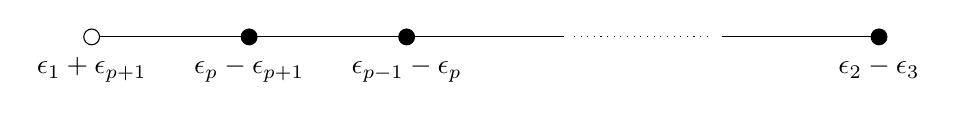
\begin{tikzpicture}
\draw (0 cm,0) -- (6 cm,0);
\draw (8 cm,0) -- (10 cm,0);
\draw[fill=white] (0 cm, 0 cm) circle (.1cm) node[below=4pt]{$\epsilon_{1} + \epsilon_{p+1}$};
\draw[fill=black] (2 cm, 0 cm) circle (.1cm) node[below=4pt]{$\epsilon_{p} - \epsilon_{p+1}$};
\draw[fill=black] (4 cm, 0 cm) circle (.1cm) node[below=4pt]{$\epsilon_{p-1} - \epsilon_{p}$};
\node (node_a) at (6 cm, 0 cm) {};
\node (node_b) at (8 cm, 0 cm) {};
\draw[fill=black] (10 cm, 0 cm) circle (.1cm) node[below=4pt]{$\epsilon_{2} - \epsilon_{3}$};
\draw [dotted] (node_a) to (node_b);
\end{tikzpicture}  
  \caption{The reduced hermitian symmetric pair $(\mathfrak{g}_\lambda, \mathfrak{k}_\lambda)$}
\end{figure}
  
The integral cone is in this case
  \[
    C = \{ a_1\omega_1 + a_{p+1}\omega_{p+1} + \cdots + a_n \omega_n \,|\, a_1 + 2( a_{p+1} + \cdots + a_{n-2}) + a_{n-1} + a_n = 0 \}
  \]
  and one can easily check that $\Psi^+_\lambda = \Psi^+_{\lambda+\mu}$ for all $\mu \in C$ and thus the translation theorem \ref{thm:translation} applies.
  
\begin{figure}[H]
  \centering
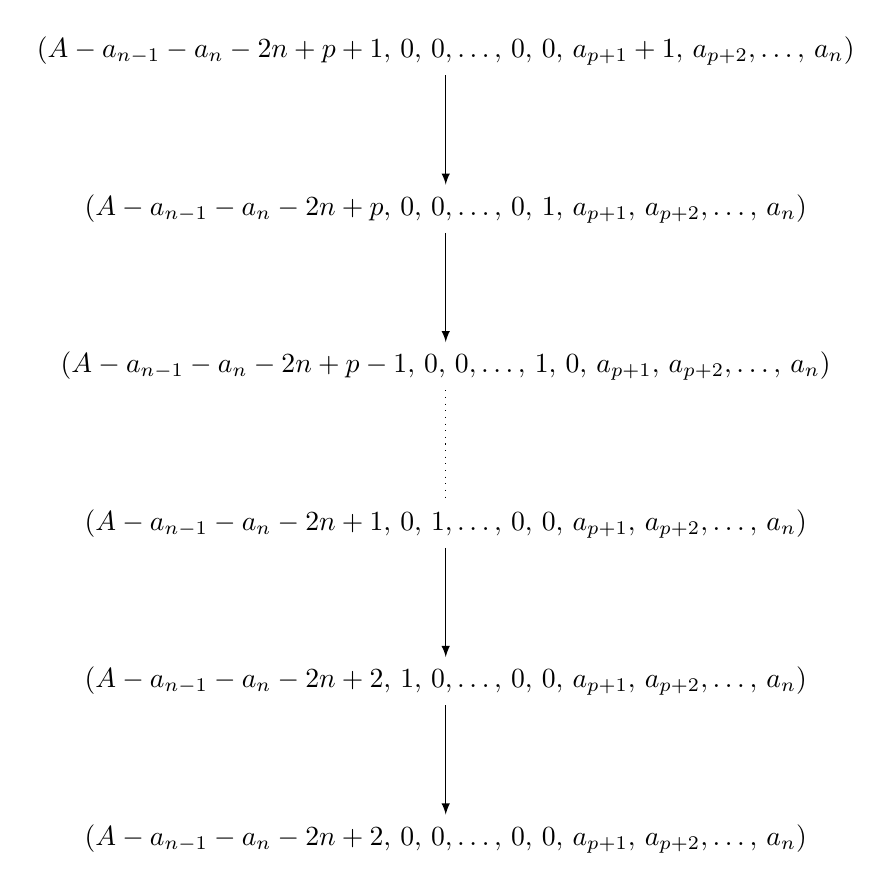
\begin{tikzpicture}[>=latex,line join=bevel,]
%%
  \node (node_0) at (0,10) [draw,draw=none] {$\left(A - a_{n-1} - a_{n} - 2n + p + 1,\,0,\,0,\ldots,\,0,\,0,\,a_{p+1}+1,\,a_{p+2},\ldots,\,a_{n}\right)$};

  \node (node_1) at (0,8) [draw,draw=none] {$\left(A - a_{n-1} - a_{n} - 2n + p,\,0,\,0,\ldots,\,0,\,1,\,a_{p+1},\,a_{p+2},\ldots,\,a_{n}\right)$};

  \node (node_2) at (0,6) [draw,draw=none] {$\left(A - a_{n-1} - a_{n} - 2n + p-1,\,0,\,0,\ldots,\,1,\,0,\,a_{p+1},\,a_{p+2},\ldots,\,a_{n}\right)$};

  \node (node_3) at (0,4) [draw,draw=none] {$\left(A - a_{n-1} - a_{n} - 2n + 1,\,0,\,1,\ldots,\,0,\,0,\,a_{p+1},\,a_{p+2},\ldots,\,a_{n}\right)$};

  \node (node_4) at (0,2) [draw,draw=none] {$\left(A - a_{n-1} - a_{n} - 2n + 2,\,1,\,0,\ldots,\,0,\,0,\,a_{p+1},\,a_{p+2},\ldots,\,a_{n}\right)$};
  
  \node (node_5) at (0,0) [draw,draw=none] {$\left(A - a_{n-1} - a_{n} - 2n +2,\,0,\,0,\ldots,\,0,\,0,\,a_{p+1},\,a_{p+2},\ldots,\,a_{n}\right)$};

  \draw [black,->] (node_0) edge (node_1);
  \draw [black,->] (node_1) edge (node_2);
  \draw [dotted] (node_2) to (node_3);
  \draw [black,->] (node_3) edge (node_4);
  \draw [black,->] (node_4) edge (node_5);
%
\end{tikzpicture}
  \caption{Nilpotent cohomology / BGG resolution, $A = -2(a_{p+1} + \cdots + a_{n-2})$}
\end{figure}
  
 \item $ \lambda = -(n+1)\omega_1 +\omega_{n-1} + \omega_n$\\
   Scalar products of positive noncompact roots with $\lambda+\rho$ 
  \begin{align*}
    (\epsilon_1 + \epsilon_j, \lambda+\rho) & = \begin{cases}
                                                 n-j, & 1<j < n \\
                                                 -1, & j = n
                                                \end{cases}\\
    (\epsilon_1 - \epsilon_j, \lambda+\rho) & = \begin{cases}
                                                 -n-2+j, & 1<j < n \\
                                                 -1, & j = n
                                                \end{cases}
  \end{align*}
  show that there are no singular roots $\Psi^+_\lambda = \emptyset$ and that the set of generating roots is $\roots^+_{n,\lambda} = \{\epsilon_1 + \epsilon_j \,|\, 1<j<n \}$. The generated root subsystem of $\roots$ is
  \[
%    \roots_\lambda = \{\pm \epsilon_i \pm \epsilon_j \,|\, i\neq j, i,j = 1,\ldots, n-1 \}.
    \roots_\lambda = \{ \pm(\epsilon_1 + \epsilon_j \,|\, 1<j < n \} \cup \{ \epsilon_i - \epsilon_j \,|\, 1 < i,j \leq n \et i\neq j \}
  \]
  and is of type $A_{n-2}$. The integral cone is
  \[
   C = \{-(a+b)\omega_1 + a\omega_{n-1} + b\omega_n) \,|\, a,b\in\mathbb{N}_0 \}
  \]
  and an easy calculation gives $\Psi^+_\lambda = \Psi^+_{\lambda+\mu}$ for all $\mu \in C$. Thus we can use the theorem \ref{thm:translation} and get the same shape of cohomology on the whole cone.
  
\begin{figure}[H]
  \centering
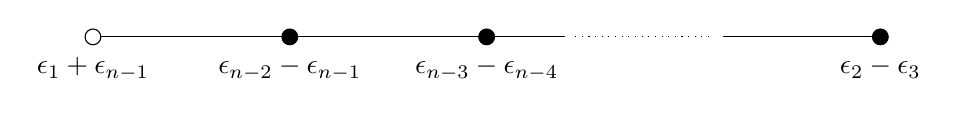
\begin{tikzpicture}
\draw (0 cm,0) -- (6 cm,0);
\draw (8 cm,0) -- (10 cm,0);
\draw[fill=white] (0 cm, 0 cm) circle (.1cm) node[below=4pt]{$\epsilon_{1} + \epsilon_{n-1}$};
\draw[fill=black] (2.5 cm, 0 cm) circle (.1cm) node[below=4pt]{$\epsilon_{n-2} - \epsilon_{n-1}$};
\draw[fill=black] (5 cm, 0 cm) circle (.1cm) node[below=4pt]{$\epsilon_{n-3} - \epsilon_{n-4}$};
\node (node_a) at (6 cm, 0 cm) {};
\node (node_b) at (8 cm, 0 cm) {};
\draw[fill=black] (10 cm, 0 cm) circle (.1cm) node[below=4pt]{$\epsilon_{2} - \epsilon_{3}$};
\draw [dotted] (node_a) to (node_b);
\end{tikzpicture}  
  \caption{The reduced hermitian symmetric pair $(\mathfrak{g}_\lambda, \mathfrak{k}_\lambda)$}
\end{figure}  

 
\begin{figure}[H]
  \centering
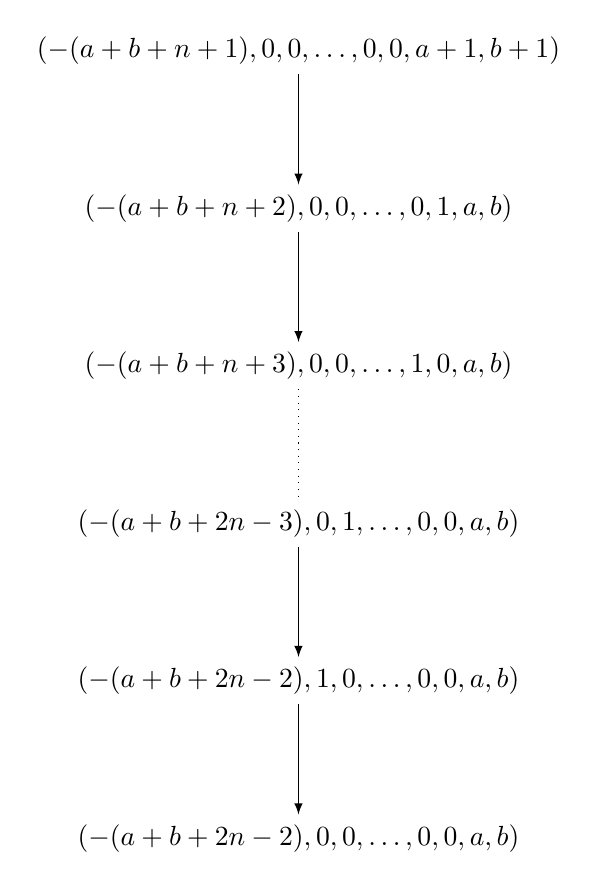
\begin{tikzpicture}[>=latex,line join=bevel,]
%%
  \node (node_0) at (0,10) [draw,draw=none] {$\left(-(a+b+n+1), 0, 0, \ldots, 0, 0, a+1, b+1 \right)$};

  \node (node_1) at (0,8) [draw,draw=none] {$\left(-(a+b+n+2), 0, 0, \ldots, 0, 1, a, b \right)$};

  \node (node_2) at (0,6) [draw,draw=none] {$\left(-(a+b+n+3), 0, 0, \ldots, 1, 0, a, b \right)$};

  \node (node_3) at (0,4) [draw,draw=none] {$\left(-(a+b+2n-3), 0, 1, \ldots, 0, 0, a, b \right)$};

  \node (node_4) at (0,2) [draw,draw=none] {$\left(-(a+b+2n-2), 1, 0, \ldots, 0, 0, a, b \right)$};
  
  \node (node_5) at (0,0) [draw,draw=none] {$\left(-(a+b+2n-2), 0, 0, \ldots, 0, 0, a, b \right)$};

  \draw [black,->] (node_0) edge (node_1);
  \draw [black,->] (node_1) edge (node_2);
  \draw [dotted] (node_2) to (node_3);
  \draw [black,->] (node_3) edge (node_4);
  \draw [black,->] (node_4) edge (node_5);
%
\end{tikzpicture}
  \caption{Nilpotent cohomology / BGG resolution}
\end{figure}
  
 \item $ \lambda = -(n-1)\omega_1 + \omega_n$\\
  Scalar products of positive noncompact roots with $\lambda+\rho$ are
  \begin{align*}
    (\epsilon_1 + \epsilon_j, \lambda+\rho) & = n+1-j\\
    (\epsilon_1 - \epsilon_j, \lambda+\rho) & = j-n.
  \end{align*}
  The integral cone is in this case \[C = \{t(-\omega_1 + \omega_n) \,|\, t\in\mathbb{N}_0 \}\] and there is a scalar product that depends on the value of $t$, namely the scalar product with the root $\epsilon_1 - \epsilon_n.$
  
  For $t=0$ we obtain set of singular roots $\Psi^+_\lambda = \{ \epsilon_1-\epsilon_n\}$ and set generating roots $\roots^+_{n,\lambda} = \{ \epsilon_1 + \epsilon_n \}$. This gives the subsystem of type $A_1$
  \[
   \roots_\lambda = \{ \epsilon_1 + \epsilon_n, -\epsilon_1 - \epsilon_n\}
  \]
  and the resulting weights for nontrivial cohomology groups are all in the table \ref{tbl:so_even}. 
  
  For $t\geq 1$ we get no singular roots $\Psi^+_\lambda = \emptyset$ and the generated subsystem is of type $A_{n-1}.$

\begin{figure}[H]
  \centering
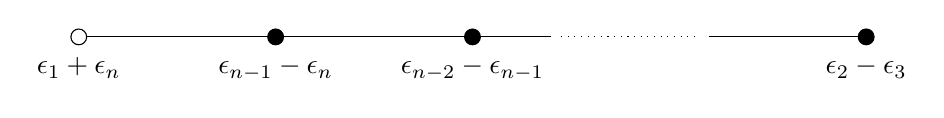
\begin{tikzpicture}
\draw (0 cm,0) -- (6 cm,0);
\draw (8 cm,0) -- (10 cm,0);
\draw[fill=white] (0 cm, 0 cm) circle (.1cm) node[below=4pt]{$\epsilon_{1} + \epsilon_{n}$};
\draw[fill=black] (2.5 cm, 0 cm) circle (.1cm) node[below=4pt]{$\epsilon_{n-1} - \epsilon_{n}$};
\draw[fill=black] (5 cm, 0 cm) circle (.1cm) node[below=4pt]{$\epsilon_{n-2} - \epsilon_{n-1}$};
\node (node_a) at (6 cm, 0 cm) {};
\node (node_b) at (8 cm, 0 cm) {};
\draw[fill=black] (10 cm, 0 cm) circle (.1cm) node[below=4pt]{$\epsilon_{2} - \epsilon_{3}$};
\draw [dotted] (node_a) to (node_b);
\end{tikzpicture}  
  \caption{The reduced hermitian symmetric pair $(\mathfrak{g}_\lambda, \mathfrak{k}_\lambda)$}
\end{figure}  

\begin{figure}[H]
  \centering
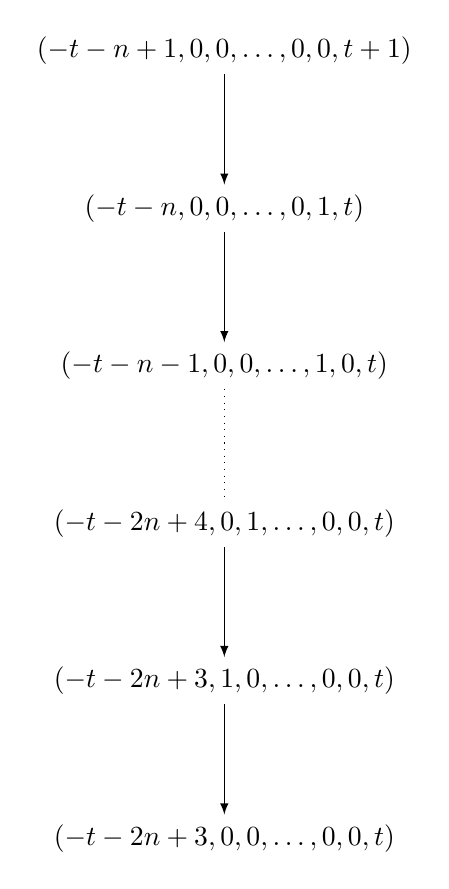
\begin{tikzpicture}[>=latex,line join=bevel,]
%%
  \node (node_0) at (0,10) [draw,draw=none] {$\left(-t-n+1, 0, 0, \ldots, 0, 0, t+1\right)$};
  \node (node_1) at (0,8) [draw,draw=none] {$\left(-t-n, 0, 0, \ldots, 0, 1, t \right)$};
  \node (node_2) at (0,6) [draw,draw=none] {$\left(-t-n-1, 0, 0, \ldots, 1, 0, t \right)$};
  \node (node_3) at (0,4) [draw,draw=none] {$\left(-t-2n+4, 0, 1, \ldots, 0, 0, t \right)$};
  \node (node_4) at (0,2) [draw,draw=none] {$\left(-t-2n+3, 1, 0, \ldots, 0, 0, t \right)$};
  \node (node_5) at (0,0) [draw,draw=none] {$\left(-t-2n+3, 0, 0, \ldots, 0, 0, t \right)$};

  \draw [black,->] (node_0) edge (node_1);
  \draw [black,->] (node_1) edge (node_2);
  \draw [dotted] (node_2) to (node_3);
  \draw [black,->] (node_3) edge (node_4);
  \draw [black,->] (node_4) edge (node_5);
%
\end{tikzpicture}
  \caption{Nilpotent cohomology / BGG resolution}
\end{figure}

 \item $ \lambda = -(n-2)\omega_1$\\
  Scalar products of positive noncompact roots with $\lambda+\rho$ are
  \begin{align*}
    (\epsilon_1 + \epsilon_j, \lambda+\rho) & = 1+n-j\\
    (\epsilon_1 - \epsilon_j, \lambda+\rho) & = 1-n+j.
  \end{align*}
  The set of singular positive roots is $\Psi^+_\lambda = \{ \epsilon_1 - \epsilon_{n-1} \}$ and the set of generating roots $\roots^+_{n,\lambda} = \{ \epsilon_1 + \epsilon_{n-1} \}$. It  follows that
  \[
   \roots_\lambda = \{\epsilon_1 + \epsilon_{n-1},-\epsilon_1 -\epsilon_{n-1} \},
  \]
  which is of type $A_1$ and all the information on cohomology is already contained in the table \ref{tbl:so_even}. %TODO opravdu je to typ A_1? Funguje prosta zmena baze?
  
 \item $ \lambda = 0$\\
  Scalar products of positive noncompact roots with $\lambda+\rho$ are given by \eqref{eq:Dn_rho_scalar_posroots} and we see that there are no singular roots $\Psi_\lambda = \emptyset$ since all scalar products are positive integers. It follows that $\roots^+_{n,\lambda} = \roots^+_n$ and after a moment of thought we realize that 
  \[
   \roots_\lambda = \roots.
  \]
  We conclude that the cohomology is in this case computed by the orginial Kostant's formula. %TODO tohle by ale bejt konecnedimenzionalni reprezentace, tak jaktoze je unitarizovatelna?
  
 \item $ \lambda = -(n-1)\omega_1  + \omega_{n-1}$\\
  Scalar products of positive noncompact roots with $\lambda+\rho$ are
  \begin{align*}
    (\epsilon_1 + \epsilon_j, \lambda+\rho) & = \begin{cases}
                                                 n+1-j, & 1<j < n \\
                                                 0, & j = n
                                                \end{cases}\\
    (\epsilon_1 - \epsilon_j, \lambda+\rho) & = \begin{cases}
                                                j-n, & 1<j < n \\
                                                 1, & j = n
                                                \end{cases}
  \end{align*}
  which gives $\Psi^+_\lambda = \{\epsilon_1 +\epsilon_n \}$ and $\roots^+_{n,\lambda} = \{\epsilon_1 - \epsilon_n \}$. This generates the roots subsystem of type $A_1$
  \[
   \roots_\lambda = \{ \epsilon_1 - \epsilon_n, \epsilon_n - \epsilon_1 \}
  \]
  and all the cohomology information is contained in table \ref{tbl:so_even}. The integral cone is in this case \[C = \{x(-\omega_1 + \omega_{n-1}) \,|\, x\in\mathbb{N}_0 \}\] and one for $\mu  \in C$, $\mu = -x\omega_1 + x\omega_{n-1}$ one has
  \begin{align*}
    (\epsilon_1 + \epsilon_j, \mu) & = \begin{cases}
                                                 0, & 1<j < n \\
                                                 -x, & j = n
                                                \end{cases}\\
    (\epsilon_1 - \epsilon_j, \mu) & = \begin{cases}
                                                -x, & 1<j < n \\
                                                 0, & j = n.
                                                \end{cases}
  \end{align*}
  Since $x$ is a positive integer, it follows that
  \[
   \Psi^+_{\lambda + \mu} = \emptyset, \quad \roots^+_{n,\lambda+\mu} = \{ \epsilon_1 - \epsilon_n \} \cup \{\epsilon_1 + \epsilon_j \,|\, 1<j<n \}.
  \]
  The root subsystem generated by reflections is
  \[
   \roots_{\lambda + \mu} = \{\pm(\epsilon_1-\epsilon_n)\} \cup \{\pm(\epsilon_1 + \epsilon_j \,|\, 1<j<n\} \cup \{ \epsilon_i - \epsilon_j \,|\, 1<i,j<n \et i \neq j\}
  \]
  and is of type $A_{n-1}$.


\begin{figure}[H]
  \centering
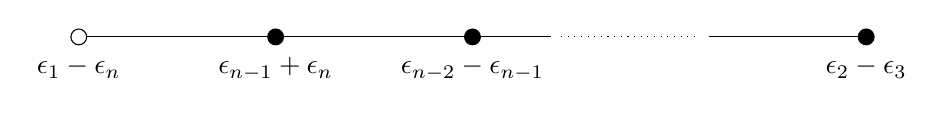
\begin{tikzpicture}
\draw (0 cm,0) -- (6 cm,0);
\draw (8 cm,0) -- (10 cm,0);
\draw[fill=white] (0 cm, 0 cm) circle (.1cm) node[below=4pt]{$\epsilon_{1} - \epsilon_{n}$};
\draw[fill=black] (2.5 cm, 0 cm) circle (.1cm) node[below=4pt]{$\epsilon_{n-1} + \epsilon_{n}$};
\draw[fill=black] (5 cm, 0 cm) circle (.1cm) node[below=4pt]{$\epsilon_{n-2} - \epsilon_{n-1}$};
\node (node_a) at (6 cm, 0 cm) {};
\node (node_b) at (8 cm, 0 cm) {};
\draw[fill=black] (10 cm, 0 cm) circle (.1cm) node[below=4pt]{$\epsilon_{2} - \epsilon_{3}$};
\draw [dotted] (node_a) to (node_b);
\end{tikzpicture}  
  \caption{The reduced hermitian symmetric pair $(\mathfrak{g}_\lambda, \mathfrak{k}_\lambda)$}
\end{figure}  

\begin{figure}[H]
  \centering
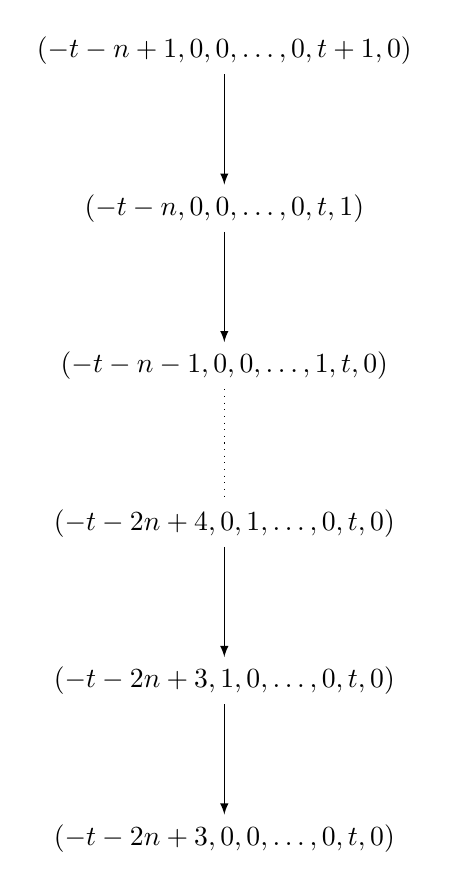
\begin{tikzpicture}[>=latex,line join=bevel,]
%%
  \node (node_0) at (0,10) [draw,draw=none] {$\left(-t-n+1, 0, 0, \ldots, 0, t+1, 0\right)$};
  \node (node_1) at (0,8) [draw,draw=none] {$\left(-t-n, 0, 0, \ldots,  0, t, 1 \right)$};
  \node (node_2) at (0,6) [draw,draw=none] {$\left(-t-n-1, 0, 0, \ldots, 1,  t, 0 \right)$};
  \node (node_3) at (0,4) [draw,draw=none] {$\left(-t-2n+4, 0, 1, \ldots, 0,  t, 0 \right)$};
  \node (node_4) at (0,2) [draw,draw=none] {$\left(-t-2n+3, 1, 0, \ldots, 0,  t, 0 \right)$};
  \node (node_5) at (0,0) [draw,draw=none] {$\left(-t-2n+3, 0, 0, \ldots, 0,  t, 0 \right)$};

  \draw [black,->] (node_0) edge (node_1);
  \draw [black,->] (node_1) edge (node_2);
  \draw [dotted] (node_2) to (node_3);
  \draw [black,->] (node_3) edge (node_4);
  \draw [black,->] (node_4) edge (node_5);
%
\end{tikzpicture}
  \caption{Nilpotent cohomology / BGG resolution}
\end{figure}


\end{enumerate}

\begin{figure}[H]
  \centering 
  \begin{tikzpicture}[>=latex,line join=bevel,]
%%
\node (alpha1) at (95bp,310bp) [draw,draw=none] {$\alpha_{1}$};
  \node (alpha1+2*alpha2+2*alpha3+alpha4+alpha5) at (95bp,8bp) [draw,draw=none] {$\alpha_{1} + 2\alpha_{2} + 2\alpha_{3} + \alpha_{4} + \alpha_{5}$};
  \node (alpha1+alpha2+alpha3+alpha4) at (43bp,161bp) [draw,draw=none] {$\alpha_{1} + \alpha_{2} + \alpha_{3} + \alpha_{4}$};
  \node (alpha1+alpha2) at (95bp,261bp) [draw,draw=none] {$\alpha_{1} + \alpha_{2}$};
  \node (alpha1+alpha2+alpha3) at (95bp,211bp) [draw,draw=none] {$\alpha_{1} + \alpha_{2} + \alpha_{3}$};
  \node (alpha1+alpha2+alpha3+alpha4+alpha5) at (95bp,111bp) [draw,draw=none] {$\alpha_{1} + \alpha_{2} + \alpha_{3} + \alpha_{4} + \alpha_{5}$};
  \node (alpha1+alpha2+2*alpha3+alpha4+alpha5) at (95bp,60bp) [draw,draw=none] {$\alpha_{1} + \alpha_{2} + 2\alpha_{3} + \alpha_{4} + \alpha_{5}$};
  \node (alpha1+alpha2+alpha3+alpha5) at (148bp,161bp) [draw,draw=none] {$\alpha_{1} + \alpha_{2} + \alpha_{3} + \alpha_{5}$};
  \draw [black,->] (alpha1) ..controls (95bp,297.84bp) and (95bp,287.19bp)  .. (alpha1+alpha2);
  \draw [black,->] (alpha1+alpha2+alpha3+alpha5) ..controls (133.01bp,146.43bp) and (119.5bp,134.19bp)  .. (alpha1+alpha2+alpha3+alpha4+alpha5);
  \draw [black,->] (alpha1+alpha2+alpha3) ..controls (109.99bp,196.43bp) and (123.5bp,184.19bp)  .. (alpha1+alpha2+alpha3+alpha5);
  \draw [black,->] (alpha1+alpha2+alpha3) ..controls (80.373bp,196.5bp) and (67.296bp,184.43bp)  .. (alpha1+alpha2+alpha3+alpha4);
  \draw [black,->] (alpha1+alpha2) ..controls (95bp,247.29bp) and (95bp,237.02bp)  .. (alpha1+alpha2+alpha3);
  \draw [black,->] (alpha1+alpha2+2*alpha3+alpha4+alpha5) ..controls (95bp,45.763bp) and (95bp,35.065bp)  .. (alpha1+2*alpha2+2*alpha3+alpha4+alpha5);
  \draw [black,->] (alpha1+alpha2+alpha3+alpha4) ..controls (57.627bp,146.5bp) and (70.704bp,134.43bp)  .. (alpha1+alpha2+alpha3+alpha4+alpha5);
  \draw [black,->] (alpha1+alpha2+alpha3+alpha4+alpha5) ..controls (95bp,97.523bp) and (95bp,86.942bp)  .. (alpha1+alpha2+2*alpha3+alpha4+alpha5);
%
\end{tikzpicture} 
	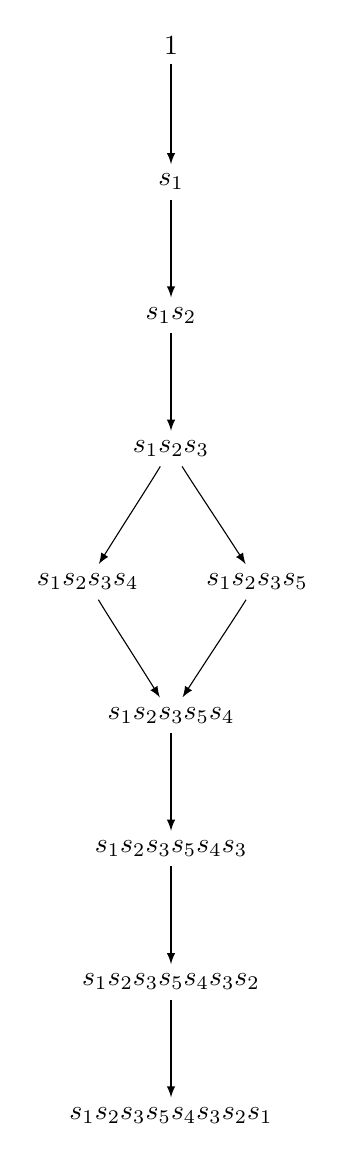
\begin{tikzpicture}[>=latex,line join=bevel,]
%%
\node (s1*s2*s3*s5*s4) at (51bp,150bp) [draw,draw=none] {$s_{1}s_{2}s_{3}s_{5}s_{4}$};
  \node (s1*s2*s3*s5*s4*s3*s2*s1) at (51bp,6bp) [draw,draw=none] {$s_{1}s_{2}s_{3}s_{5}s_{4}s_{3}s_{2}s_{1}$};
  \node (s1) at (51bp,342bp) [draw,draw=none] {$s_{1}$};
  \node (s1*s2*s3*s5*s4*s3*s2) at (51bp,54bp) [draw,draw=none] {$s_{1}s_{2}s_{3}s_{5}s_{4}s_{3}s_{2}$};
  \node (1) at (51bp,391bp) [draw,draw=none] {$1$};
  \node (s1*s2*s3) at (51bp,246bp) [draw,draw=none] {$s_{1}s_{2}s_{3}$};
  \node (s1*s2) at (51bp,294bp) [draw,draw=none] {$s_{1}s_{2}$};
  \node (s1*s2*s3*s5*s4*s3) at (51bp,102bp) [draw,draw=none] {$s_{1}s_{2}s_{3}s_{5}s_{4}s_{3}$};
  \node (s1*s2*s3*s5) at (82bp,198bp) [draw,draw=none] {$s_{1}s_{2}s_{3}s_{5}$};
  \node (s1*s2*s3*s4) at (21bp,198bp) [draw,draw=none] {$s_{1}s_{2}s_{3}s_{4}$};
  \draw [black,->] (s1*s2*s3*s5*s4) ..controls (51bp,137.55bp) and (51bp,127.07bp)  .. (s1*s2*s3*s5*s4*s3);
  \draw [black,->] (s1*s2*s3*s5*s4*s3*s2) ..controls (51bp,41.554bp) and (51bp,31.067bp)  .. (s1*s2*s3*s5*s4*s3*s2*s1);
  \draw [black,->] (1) ..controls (51bp,377.83bp) and (51bp,367.21bp)  .. (s1);
  \draw [black,->] (s1*s2*s3) ..controls (58.994bp,233.14bp) and (66.747bp,221.63bp)  .. (s1*s2*s3*s5);
  \draw [black,->] (s1*s2*s3) ..controls (43.309bp,233.21bp) and (35.918bp,221.87bp)  .. (s1*s2*s3*s4);
  \draw [black,->] (s1*s2*s3*s4) ..controls (28.691bp,185.21bp) and (36.082bp,173.87bp)  .. (s1*s2*s3*s5*s4);
  \draw [black,->] (s1) ..controls (51bp,329.55bp) and (51bp,319.07bp)  .. (s1*s2);
  \draw [black,->] (s1*s2*s3*s5*s4*s3) ..controls (51bp,89.554bp) and (51bp,79.067bp)  .. (s1*s2*s3*s5*s4*s3*s2);
  \draw [black,->] (s1*s2) ..controls (51bp,281.55bp) and (51bp,271.07bp)  .. (s1*s2*s3);
  \draw [black,->] (s1*s2*s3*s5) ..controls (74.006bp,185.14bp) and (66.253bp,173.63bp)  .. (s1*s2*s3*s5*s4);
%
\end{tikzpicture} 
  \caption{Poset of noncompact roots and the BGG graph for $\mathrm{SO}(2,8)$}
\end{figure} 
